\documentclass[a4paper]{report}
\usepackage{graphicx}
\usepackage{listings}
\usepackage{tikz}
\usepackage{amsmath}

\lstset{
    literate=%
        {č}{{\v{c}}}1
        {š}{{\v{s}}}1
        {ž}{{\v{z}}}1
        {λ}{{$\lambda$}}1
}

\title{diploma}
\author{Luka Sabotic}
\date{August 2023}

\begin{document}

\maketitle

\section{Povzetek}
\newpage

\section{Uvod}
1 stran
\newpage

\section{Teorija}
10 strani

todo: 
- mi notacija, fix operator
- <> oklepaji
- prevedi equi in iso recursive
- prevedi sum types
- right arrows inside code blocks
- prevod enumerations in single field variants
- eval.ml, kaj to dela in ali je sploh uporabno. če je, popravi še število filov, ki sestavljajo Minihaskell

A hočem tud 'podatkovni tipi'? -> mogoče v uvodu?

- RECURSIVE TYPES:  	20 - recursive types: examples, formalities

                        (processes ?), hungry functions, streams

    	            	21 - induction, finite and infinite

                        equi-recursive and iso-recursive

- CASE: 

        sums, variants -  11.9, 11.10

        how if is 'compiled' into case

\section{Implementacija}
15 strani

vsi fili, kaj kšn file dela, kaj je blo treba spremenit

(kaj bi lahko izbrisal)

- TIPI:

- CASE:

\section{Uporaba}
10 strani

- Menjava vseh tipov z impementiranimi

lists: 20.1 kar dobro pove kaj vse rabiš za delo s seznami - to lahko pokažem, enako lahko mogoče nardim za drevesa

- rekurzivni tipi: seznami, drevesa, ...

stream:

data Stream = Cons Int Stream

let ones = rec ones : Stream is Cons 1 ones

podobno poiskusi z ostalimi 'hungry' funkcijami

- Zanimivi rekurzivni tipi

- funkcije z uporabo case


\newpage
\section{Rekurzivni tipi} %zaenkrat 1 stran plus razlaga primera seznama z drevesom -> cca 1.5 strani 
V programiranju se vsakodnevno srečujemo z velikim številom konceptov in idej, ki nam na različne načine omogočajo iskati rešitve. Eden najbolj osnovnih in popularnih je tudi rekurzija.
V osnovi rekurzija predstavlja elegantno preprostost reševanja zapletenih problemov z razčlenitvijo na manjše, bolj obvladljive podprobleme. Ta sposobnost reševanja zapletenih izzivov 
postopoma, ni le preoblikovala načina, kako se programerji lotevajo kodiranja, temveč je tudi postavila temelje za ustvarjanje razreda podatkovnih struktur, imenovanih rekurzivni tipi.

Tako kot rekurzivna funkcija pokliče samo sebe, da reši problem v manjših korakih, rekurzivni tipi opredeljujejo strukture, ki vsebujejo elemente istega tipa in ustvarjajo strukturirane 
samo-referenčne vzorce. S tem, ko dovoljujejo, da so elementi strukture sestavljeni iz primerkov iste strukture, oponašajo naraven način, kako zaznavamo in opisujemo svet okoli nas. 
Na primer datotečni sistem, kjer lahko mape vsebujejo podmape, ki pa spet vsebujejo več map in datotek. Podobno v družinskem drevesu: posamezniki imajo otroke, ki sčasoma sami 
postanejo starši. Rekurzivni tipi omogočajo, da te kompleksne odnose opišemo na preprost in intuitiven način.

Rekurzivni tip je podatkovni tip, ki se v svoji definiciji sklicuje sam nase. Ločimo ji lahko na induktivne in koinduktivne tipe. Prvi so končni, drugi pa so lahko tudi neskončni. 
Morda najbolj osnoven primer rekurzivnega tipa, je seznam. Seznam je lahko prazen, ali pa vsebuje urejen par nekega elementa in drugega seznama. Elementu ponavadi rečemo glava, seznamu, 
ki glavi sledi, pa rep. Tako ima poljubno dolžino, lahko je tudi prazen. Njegovo definicijo zapišemo kot:
\begin{lstlisting}
    List = <nil:Unit, cons:{Element, List}>
\end{lstlisting}
kjer \emph{nil} prestavlja odsotnost vrednosti, torej prazen seznam. V prikazovanju primerov svoje implementacije bom za prazen seznam uporabljal konstruktor \emph{Empty}, 
ki ne sprejme nobenega argumenta. \emph{Element} pa predstavlja vrednost, ki je vsebovana v seznamu. Ta je seveda odvisna od tipa seznama. Če bi na primer hoteli seznam celih števil, 
bi definicija izgledala tako:
\begin{lstlisting}
    ListInt = <nil:Unit, cons:{Int, ListInt}>
\end{lstlisting}
v moji impementaciji v Minihaskellu pa bi to izlgedalo kot:
\begin{lstlisting}
    data ListInt = Empty | Cons Int ListInt
\end{lstlisting}
Primer seznama celih števil, ki vsebuje elemente 1, 2 in 3:
\begin{lstlisting}
    let oneToThree = Cons 1 (Cons 2 (Cons 3 Empty))
    > val oneToThree : ListInt
\end{lstlisting}

Ta seznam si lahko predstavljamo tudi kot drevo:

\begin{center}
    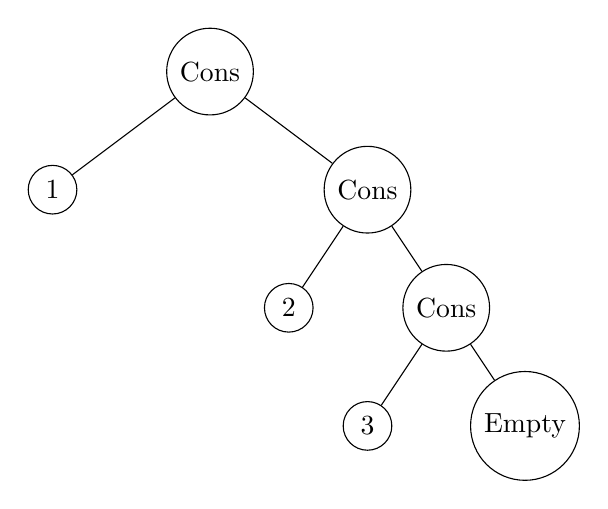
\begin{tikzpicture}[
        level 1/.style={sibling distance=40mm},
        level 2/.style={sibling distance=20mm},
        node/.style={circle, draw, minimum size=5mm}
      ]
      \node[node] {Cons}
        child {
          node[node] {1}
        }
        child {
          node[node] {Cons}
          child {
            node[node] {2}
          }
          child {
            node[node] {Cons}
            child {
              node[node] {3}
            }
            child {
              node[node] {Empty}
            }
          }
        };
      \end{tikzpicture}
\end{center}

Različne vrednosti, ki jih lahko zavzame rekurzivni tip predstavimo s konstruktorji, ki sprejmenjo neko število argumentov, ki so lahko spet kostruktorji. V drevesnem prikazu tega tipa so 
konstruktorji vozlišča, argumenti pa njihovi otroci. Konstruktorji, ki ne sprejmejo nobenih argumetnov, na primer \emph{Empty}, so listi drevesa. V našem primeru seznama s števili 
ena do tri, poznamo dva konstruktorja: \emph{Cons} in \emph{Empty}. Drevo ima tudi liste, ki predstavljajo števila. Torej lahko podan primer razčlenimo:
\begin{enumerate}
    \item imamo seznam, ki vsebuje število 1 in nek drug seznam ali rep. Konstruktor, ki nam omogoča to strukturo je \emph{Cons}, ki sprejme dva argumenta: število in seznam. To sta 
    njegova otroka. Vzamemo torej prvi del definicije: \textbf{Cons 1 rep}.
    \item Seznam, ki je 'rep' seznama s številom 1, je spet seznam, ki vsebuje število 2 in nov seznam. Spet uporabimo konstruktor \emph{Cons} in mu podamo argumenta 2 in nov seznam, se pravi 
    \textbf{Cons 2 rep}.
    \item Ostane nam še število 3, ki ga kot argument ponudimo tretjemu \emph{Cons} konstruktorju. Potrebujemo še repni seznam: \textbf{Cons 3 rep}.
    \item Ker smo na koncu seznama, uporabimo konstruktor \textbf{Empty} in zaključimo strukturo.
\end{enumerate}

Seznamom podoben primer so drevesa. Ta so sestavljena iz vozlišč, vsako je lahko prazno, ali pa vsebuje nek element in svoje otroke. Ti so spet drevesa. V svetu programiranja so seznami in drevesa 
ključne podatkovne strukture, ki jih uporabljamo na različne načine. Razvijajo se inovativne implementacije in algoritmi za delo z njimi in so nujni za razumevanje programiranja.
Seveda pa so to hkrati le osnovni primeri rekurzivnih tipov. V nadaljevanju bom predstavil nekaj bolj zanimivih primerov, ki so prav tako zelo uporabni.

\subsection{Koinduktivni podatkovni tipi}
Seznami in drevesa so končni rekurzivni tipi, kar je lako zelo prikladno, ker lahko hranimo njihovo celo vsebino. Lahko pa se zgodi, da porebujemo podatkovni tip, ki nam omogoča dostop do 
neomejene količine podatkov. Tu nastopijo koinduktivni tipi. Najbolj so povezani z uporabo v komunikacijah, kjer ni potrebe da se komunikacijaski kanal kdaj zapre, najdemo pa jih lahko v  
postopkih, ki so lahko neskončni. 

Osnovni primer koinduktivnih tipov so lačne funkcije. To so funkcije, ki sprejmejo poljubno število argumentov in vrnejo novo funkcijo, ki je lačna novih argumentov:
\begin{equation}
    \text{Lačna} = \mu X. (\text{Argument} \rightarrow X) \notag
\end{equation}
Na primer, lahko imamo funkcijo, ki sprejme število in vrne funkcijo, ki sprejme novo število:
\begin{lstlisting}
    f = fix (λf:Int->Lačna. λn:Int. f)
    > f : Lačna
\end{lstlisting}
Ko jo polkičemo, bo vrnila novo funkcijo, ki bo lačna novih argumentov:
\begin{lstlisting}
    l_1 = f 1;
    > l_1 : Lačna
\end{lstlisting}
Rezultatu lahko nato podamo nov argument in dobili bomo enak rezultat:
\begin{lstlisting}
    l_2 = l_1 2;
    > l_2 : Lačna  
\end{lstlisting}
Tako funkcijo lahko gledamo tudi kot funkcijo, ki sprejme neomejeno količino argumentov in še vedno bo lačna novih:
\begin{lstlisting}
    zelo_lačna = f 1 2 3 4 5 6 7 8 9 10;
    > zelo_lačna : Lačna
\end{lstlisting}
V resnici je \emph{zelo\_lačna} sestavljena iz več lačnih funkcij, ki se poračunajo sproti z vsakim argumentom. Lahko bi jo zapisali tudo kot:
\begin{lstlisting}
    zelo_lačna = (((((((((f 1) 2) 3) 4) 5) 6) 7) 8) 9) 10
    > zelo_lačna : Lačna
\end{lstlisting}
Tako se 1 uporabi kot argument na funkciji f, 2 na funkciji, ki jo vrne f, ko sprejme 1 in tako naprej.

Koinduktivni tipi so torej zelo uporabni, ker nam omogočajo delo z neskončnimi podatki. Vendar pa je potrebno biti previden, ker lahko hitro pride do neskončnih zank, ki se nikoli ne izračunajo. 
Lažje jih je obvladovati v lenih programskih jezikih, ker se njihova vsebina nikoli ne izračuna do konca, vedno samo po potrebi.

Najbolj znane lačne funkcije so \emph{tokovi}. To so funkcije, ki sprejmejo prazne vrednosti (\emph{Unit}) in vrnejo pare elementov in novih tokov:
\begin{equation}
    Tok = \mu X. (Unit \rightarrow {Element, X}) \notag
\end{equation}
Lažji način za razumevanje tokov je, da jih gledamo kot neskončne sezname, sestavljene iz parov elementov in novih tokov. Na primer, lahko imamo tok naravnih števil:
\begin{lstlisting}
    naravna = fix (λf:Int->Tok. λn:Int. λu:Unit. 
        {n, f (n+1)}) 0;
    > naravna : Tok
\end{lstlisting}
Za delo s tako funkcijo potrebujemo še nekaj pomožnih funkcij. Najprej funkcijo, ki vrne prvi element, ali glavo toka: (imejmo 1 za indeks prvega elementa in 2 za indeks drugega)
\begin{lstlisting}
    glava = λt:Tok. (t Unit).1;
    > Tok : Tok -> Int
\end{lstlisting}
in še funkcijo, ki vrne rep toka:
\begin{lstlisting}
    rep = λt:Tok. (t Unit).2;
    > rep : Tok -> Tok
\end{lstlisting}
Tako lahko dostopamo do poljubnega elementa v toku:
\begin{lstlisting}
    tri = glava (rep (rep (rep naravna)));
    > 3 : Int
\end{lstlisting}

Oglejmo si še nadgradnjo tokov, enostavne procese. To so funkcije, ki sprejmejo nek element in vrnejo par elementa in novega procesa:
\begin{equation}
    Proces = \mu X. (Element \rightarrow {Element, X}) \notag
\end{equation}
Na primer, lahko imamo proces, ki sproti vrača XOR zadnjih dveh prejetih elementov:
\begin{lstlisting}
    xor = fix (λf:Bool->Proces. λb_1:Bool. λb_2:Bool. 
        let new_b = xor b_1 b_2 in
        {new_b, f new_b}) true;
    > xor : Proces
\end{lstlisting}
Podobno kot pro tokovih, za delo s procesi potrebujemo pomožne funkcije, kot je na primer funkcija, ki vrne vrnjeno vrednost procesa:
\begin{lstlisting}
    vrednost = λp:Proces. (p true).1;
    > vrednost : Proces -> Bool
\end{lstlisting}


\subsection{Equi-recursive ali Iso-recursive?}
Ko implementiramo rekurzivne tipe, se moramo slej ko prej vprašati, kaj je razlika med tipom in čemer dobimo, ko ta tip enkrat 'odvijemo'. Na primer, kaj je razlika med tipom \emph{List}
in njegovim enkratnim odvojem \emph{<nil:Unit, cons:{Element, List}>}? V literatiri pojavita dva pristopa k temu vprašanju: \emph{equi-recursive} in \emph{iso-recursive}.
\subsubsection{Equi-recursive}
Equi-recursive pristop pravi, da je tip \emph{\(\mu\)X.F(X)} po definiciji enak njegovemu odvoju \emph{F(\(\mu\)X.F(X))}, ker oba predstavljata enaka neskončna drevesa. Ta pristop nato od 
preverjevalnika tipov zahteva, da poskrbi, da se lahko oba zapisa uporabljata kot argumenta v funkcijah in podobno.

\subsubsection{Iso-recursive}
Iso-recursive način, pa ubere na prvi pogled nekoliko bolj zapleteno pot. Definira dve preslikavi, ki sta med seboj inverzni. Imenujmo ju \emph{fold} in \emph{unfold}. Preslikava 
\emph{unfold} vzame rekurzivni tip in ga preslika v njegov prvi odvoj, torej vzame tip \(\mu\)X.T in v telesu T zamenja vse pijavitve X z celotnim rekurzivnim tipom. Na primer, v definiciji 
seznama: 
\begin{equation}
    \mu \text{List.}<\text{nil:Unit, cons:}\{\text{Element, List}\}> \notag
\end{equation}
preslikamo v
\begin{equation}
    <\text{nil:Unit, cons:}\{\text{Element,} \mu \text{List.}<\text{nil:Unit, cons:}\{\text{Element, List}\}>\}>. \notag
\end{equation}
  
\emph{Fold} pa stori ravno obratno, torej rekurzivni tip zavije nazaj. Definiciji teh preslikav lahko tako zapišemo kot:
\begin{gather}
    unfold[\mu X.T]: \mu X.T \rightarrow [X \rightarrow \mu X.T] T \notag\\
    fold[\mu X.T]: [X \rightarrow \mu X.T] T \rightarrow \mu X.T \notag
\end{gather}
Ker sta preslikavi inverzni, velja:

\begin{center}
\includegraphics[width=0.5\textwidth]{fold_unfold.jpg}
\end{center}

Tako iso-recursive pristop rekurzivni tip in njegove odvoje ne obravnava kot enake, temveč kot izomorfne.

Oba pristopa se uporabljata pri konstrukciji programskih jezikov in teoretičnih besedilih. Equi-recursive je bolj intuitiven, vednar zahteva več dela od preverjevalnika tipov in 
lahko privede do težav pri kombinaciji z drugimi konstrukti, na primer operatorjih na tipih. Medtem iso-recursive pristop zahteva uporabo preslikav \emph{fold} in \emph{unfold}, kjerkoli 
se uporabijo rekurzivni tipi. V svoji implementaciji sem uporabil equi-recursive pristop, ker je bolj intuitiven in ne zahteva uporabe dodatni preslikav. Ker je Minihaskell len programski 
jezik, preverjevalnik tipov čaka na potrebo po preverjanju tipov, kar pomeni, da se lahko uporabijo rekurzivni tipi, ne da bi jih bilo treba najprej razviti.

\section{Vsote in variante}
Programerji se pogosto srečujejo z različnimi strukturami ali spremenljivkami, ki lahko zavzamejo vrednosti iz množice opcij. Na primer, vozlišče v drevesu je lahko prazno, list, ali 
notranje vozlišče. Element v povezanem seznamu je lahko trivialna vrednost nil, ali pa vozlišče Cons z glavo in repom seznama. Takih primerov je ogromno. Zato poznamo "sum types".

\subsection{Vsote}
Vsote so tipi, ki izvirajo iz množice vrednosti, dobljene iz kombinacije natanko dveh tipov. Na primer, če imamo tipa
\begin{lstlisting}
    Odrasel = {starost: Int, izobrazba: String}
    Otrok = {starost: Int, šola: String}
\end{lstlisting}
za opis odraslega in otroka in želimo obravnavati oba kot en tip, da bi lahko na primer naredili seznam, ki vključuje oba tipa, lahko definiramo vsoto
\begin{lstlisting}
    Oseba = Odrasel + Otrok.
\end{lstlisting}
Vsak element s tipom oseba, je tipa Odrasel, ali pa Otrok.

Za ločevanje med elementi vsote, bomo uporabljali označbe \emph{inl} in \emph{inr}. Označbi prideta iz angleških izrazov \textit{inject left} in \textit{inject right}. Lahko ju razumemo kot
funkciji, v tem primeru:
\begin{gather}
    inl: Odrasel \rightarrow Oseba \notag\\
    inr: Otrok \rightarrow Oseba \notag
\end{gather}
vendar ju bomo uporabljali zgolj kot oznaki za ločevanje med elementi vsote. Torej, elementi tipa \emph{Oseba} so bodisi oblike \emph{inl x}, kjer je x tipa \emph{Odrasel}, ali pa \emph{inr y}, kjer je y 
tipa \emph{Otrok}. Torej, če je \emph{od} tipa \emph{Odrasel}, je \emph{inl od} tipa \emph{Oseba}, če pa je \emph{ot} tipa \emph{Otrok}, je \emph{inr ot} tipa \emph{Oseba}.

Da lahko nato delamo z vsotami, moramo imeti funkcije, ki znajo ločevati med elementi vsote in jih obravnavati posebej. To naredimo z uporabo \emph{case} izraza. Če nas na primer zanimajo 
informacije o izobrazbi obravnavane osebe, lahko definiramo funkcijo izobrazba:
\begin{lstlisting}
    izobrazba: λo:Oseba.
        case o of
            inl x -> x.izobrazba
            inr y -> y.šola;
\end{lstlisting}
Ko je argument o tipa Odrasel označen z \emph{inl}, se izvede prva veja in vrne izobrazba odraslega, ko pa je argument o tipa Otrok označen z \emph{inr}, se izvede druga veja in vrne šola
otroka. Tako je tip celotne funkcije \emph{Oseba $\rightarrow$ String}.

Preverjevalnik tipov tukaj nima težke naloge. Če imamo vsoto tipov \(T_1 + T_2\) in želimo pokazati, da je \emph{inl $t_1$} tipa \emph{$T_1 + T_2$}, moramo le pokazati, da je 
\emph{$t_1$} tipa \emph{$T_1$}. Podobno velja za \emph{inr $t_2$}. Za \emph{case} moramo preveriti več stvari. Najprej, da je argument tipa \emph{$T_1$ + $T_2$}. Nato preverimo 
obe veji, kjer predpostavimo da sta arumenta \emph{x} in \emph{y} tipov \emph{$T_1$} in \emph{$T_2$}, v tem vrstnem redu. Preverjamo, da sta tipa \emph{$T_1$} in \emph{$T_2$} 
vrnjenih vrednosti enaka. Če je to res, označimo tip vrnjene vrednosti kot \emph{T}. Celoten izraz ima nato tip \emph{$T_1 + T_2$ $\rightarrow$ T}.

Ker v \emph{case} izrazu preverjamo tip izraza, ki je podan kot argument na način, da samo preverimo ali ustreza enemu od \emph{\(T_1\) in \(T_2\)} in se ne oziramo na drugi tip v vsoti, 
se lahko zgodi, da je izrazu možno dodeliti več kot en tip. To se zgodi, če ima več vsot enak seštevanec. Za primer vzemimo vsoti \emph{$\alpha$ + $\beta$} in \emph{$\gamma$ + $\beta$}.
Obema je skupen seštevanec \emph{$\beta$}, torej lahko nekemu izrazu tipa \emph{$\beta$} dodelimo tip \emph{$\alpha$ + $\beta$} ali pa \emph{$\gamma$ + $\beta$}. To je problem, ki ga
lahko rešujemo na različne načine. V svoji implementaciji, sem se odločil, da bo prevajalnik tipov izbral prvi tip, ki ga najde, torej tistega, ki je bil nazadnje definiran. To je bila 
najpreprostejša rešitev, vendar onemogoča, da bi v tem primeru tip \emph{$\beta$} kakorkoli prepoznal kot del vsote \emph{$\alpha$ + $\beta$}.

\subsection{Variante}
Binarne vsote lahko razširimo na variante, ki so kot vsote s poljubnim številom seštevancev. Zato označbi \emph{inl} in \emph{inr} ne prideta več v poštev, temveč uporabimo svoje oznake. 
Tako se malenkost spremeni notacija. Namesto \emph{$T_1 + T_2$} pišemo \emph{<$l_1:T_1, ... , l_n:T_n$>}, kjer \(l_i\) stoji za i-to oznako, ali 'label'. Prav tako namesto \emph{inl t as 
$T_1 + T_2$}, pišemo \emph{<$l_1$ = t> as <$l_1:T_1, ... , l_n:T_n$>}. Tako naš primer z osebami postane:
\begin{lstlisting}
    Oseba = <odrasel:Odrasel, otrok:Otrok>;
    o = <odrasel=od> as Oseba;
    > o : Oseba

    izobrazba: λo:Oseba.
        case o of
            <odrasel = od> -> od.izobrazba
          | <otrok = ot> -> ot.šola;
    > izobrazba : Oseba -> String
\end{lstlisting}


Morda zanimiva skupina variant so tiste, ki lahko vsebujejo tudi trivialne vrednosti \emph{unit}:
\begin{lstlisting}
    Optional =  <none:unit, some:Val>;
\end{lstlisting}
Ti tipi so izomorfni s tipi, ki spadajo pod oznako \emph{some} in razširjeni z opcijo trivialne vrednosti. To so na primer tipi, ki jih poznamo iz priljubljenih programskih jezikov in dopuščajo 
vrednosti kot so \emph{null}, \emph{None} ali \emph{nil}.

Še dve posebni vrsti variant sta dovolj zanimivi za posebno obravnavo.

\subsubsection{Oštevilčenja (enumerations)}
Oštevilčenja so variante, ki vsebujejo zgolj trivialne vrendosti in so namenjene predstavljanju konstant. Na primer, če želimo predstaviti ocene, ki jih lahko dobi študent, definiramo varianto:
\begin{lstlisting}
    Ocena = <pet:Unit, šest:Unit, sedem:Unit, osem:Unit, 
            devet:Unit, deset:Unit>;
\end{lstlisting}
Elementi takega tipa bi nato bili oblike \emph{<deset=unit> as Ocena}. Tako lahko sestavimo tudi funkcije, ki obravnavajo take vrendnosti. Na primer;
\begin{lstlisting}
    možno_zviševanje = λ.o:Ocena.
        case o of 
              <deset=x> -> false
            | _         -> true;
\end{lstlisting}
je funkcija, ki sprejme eno izmed ocen in vrne odgovor na vprašanje, če jo je možno izboljšati. Tip te funkcije je \emph{Ocena $\rightarrow$ Bool}.

\subsubsection{Variante enega tipa (Single-field variants)}
Možno je ustvariti tudi variante s samo eno oznako, torej bodo vsi njeni elementi istega tipa:
\begin{lstlisting}
    V = <l:T>;
\end{lstlisting}
torej tipa \emph{T}. To je lahko zelo uporabno, ker elementov tipa \emph{V} ni možno zamešati za elemente tipa \emph{T} in posledično na njih ne moremo izvajati operacij, ki jih lahko na tipu 
\emph{T}. Tako se lahko izognemu nesmiselnim primerom. Recimo, da uporabljamo podatke o valutah. Količino denarja v posamezni valuti lahko predstavimo s tipom \emph{Float}, kot decimalno 
število. Težava nastane, ko definiramo funkcijo, ki pretvarja med valutami:
\begin{lstlisting}
    KuneVEvre = λx:Float. zmnoži x 0.1327;
    > KuneVEvre : Float -> Float
\end{lstlisting}
kjer \emph{zmnoži} predstavlja funkcijo, ki pomnoži dve decimialni števili. Če je \emph{x}, ki ga podamo funkciji \emph{KuneVEvre} količina denarja v evrih, je vse v redu. Vendar pa nam nič ne 
preprečuje, da bi kot argument v \emph{KuneVEvre} podali katerokoli drugo število, na primer količino denarja v dolarjih, ali še huje, število število komarjev v nekem prostoru. Taka uporaba te 
funkcije je nesmiselna in se ji v večini primerov želimo izogniti. Tako lahko definiramo variante enega tipa:
\begin{lstlisting}
    DenarVKunah = <kune:Float>;
    DenarVEvrih = <evri:Float>;
\end{lstlisting}
in morda še vse ostali, ki jih potrebujemo, ter funkcijo \emph{KuneVEvre} spremenimo tako, da deluje s pravilnimi tipi, torej pretvorbo omogočimo 
samo iz kun v evre in nič drugega:
\begin{lstlisting}
    KuneVEvre = λx:DenarVKunah.
        case x of 
            <kune:x> -> <evri = zmnoži x 0.1327> 
                        as DenarVEvrih;
    > KuneVEvre : DenarVKunah -> DenarVEvrih.
\end{lstlisting}
Tako se zavarujemo pred napakami.
\newpage

\section{Implementacija}
Predstavljene konstrukte sem tudi sam implementiral. To sem storil v programskem jeziku Minihaskell, ki ga je ustvaril prof. dr. Andrej Bauer in 
je dostopen na njegovem Github profilu, v repozitoriju \emph{plzoo}. 

Minihaskell je programski jezik, ki je namenjen predstavitvi osnovnih konceptov funkcionalnega programiranja. Napisan je v programskem jeziku 
OCaml in je v svojih omejitvah podoben jeziku Haskell. Omogoča uporabo celih števil (integers), booleanov z logičnimi operacijami in primerjavami 
celih števil ('=', '<'), urejenih parov, seznamov, funkcij in rekurzije. Temu sem dodal možnost definiranja novih tipov, rekurzivnih ali ne, in 
uporabe \emph{case} izrazov. Programski jezik sestavlja šest datotek, katerih namen predstavljam v naslednjih poglavjih.

\subsection{lexer.mll}
Lekser je datoteka, kjer so shranjeni regularni izrazi, ki opisujejo žetone, ki jih lahko uporabljamo v programskem jeziku. To so vse ključne 
besede, ki jih lahko uporabimo, števila, znaki, \emph{eof} in podobno. Kot je to storjeno v Haskellu, sem določil, naj bodo imaena spremenljvk 
možna le z majhno začetnico, konstruktorji in imena tipov, pa z veliko. Dodati sem moral tudi žetone za ključne besede \emph{data}, \emph{case}, 
\emph{of} in \emph{end}. Ker Minihaskell ni občutljiv na zamik vrstic v kodi, sem za lažjo interpetacijio \emph{case} izrazov dodal tudi \emph{end} 
žeton. Zakaj, si poglejmo naslednji primer. Recimo, da imamo \emph{case} izraz, ki v eni od vej vsebuje še en \emph{case} izraz:
\begin{lstlisting}
    case x of 
        a -> _
        b -> case y of
                c -> _
                d -> _
        e -> _
\end{lstlisting}
Če bi bil Minihaskell občutljiv na zamik vrstic, bi bil zgornji izraz samoumeven. Tako pa ga lahko razumemo na dva načina:
\begin{lstlisting}
    case x of 
        a -> _
        b -> case y of
                c -> _
                d -> _
        e -> _
\end{lstlisting}
ali pa:
\begin{lstlisting}
    case x of 
        a -> _
        b -> case y of
                c -> _
        d -> _
        e -> _.
\end{lstlisting}
Ker imajo različni programerji različna mnenja o tem, kaj je bolj smiselno, sem dodal \emph{end} žeton, ki nam omogoča, da nedvoumno določimo, 
kdaj se \emph{case} izraz konča:
\begin{lstlisting}
    case x of 
        a -> _
        b -> case y of
                c -> _
                d -> _
                end
        e -> _
    end.
\end{lstlisting}

\subsection{parser.mly}
Parser je naslednji korak v procesu prevajanja. Lekser posreduje tok žetonov, ki jih je prepoznal, naloga parserja pa je prepoznati sintaktično
pravilne stavke in zgraditi abstraktna sintaktična drevesa. To stori s pomočjo gramatičnih pravil, ki povejo, v kakšnem zaporedju pričakujemo 
žetone in kje se ti lahko pojavijo. V svoji implementaciji sem dodal dve gramatični pravili: eno za definicijo novih tipov in eno za \emph{case}
izraz. Pravilo za definicijo novih tipov je sledeče:
\begin{lstlisting}
    datadef:
  | DATA CNAME EQUAL data_variants { DataDef ($2, $4) },
\end{lstlisting}
ki omogoča definicijo tipov na način:
\begin{lstlisting}
    data Type = Constr 1 | Constr 2 | ... | Constr n.
\end{lstlisting}
Definicijo tipov sem definiral kot enega izmed štirih osnovnih ukazov. Pred njim so bili že definirani \emph{lettop}, ki omogoča inicializacijo 
spremenljivk, \emph{exprtop}, ki omogoča definicijo izrazov in \emph{cmdtop}, ki vsebuje posebne ukaze, kot so na primer \emph{quit}.

Pravilo za \emph{case} izraz pa je: 
\begin{lstlisting}
    expr:
    ...
    | CASE expr OF cases END { Case ($2, $4) }
\end{lstlisting}
in omogoča uporabo \emph{case} izrazov, kot so:
\begin{lstlisting}
    case x of 
        Constr 1 -> _
        Constr 2 -> _
        ...
        Constr n -> _
    end.
\end{lstlisting}
Uporabljajo se lahko le v izrazih, pod katere spadajo tudi funkcije.

\subsection{syntax.ml}


\subsection{interpret.ml}

\subsection{typecheck.ml}

\subsection{minihaskell.ml}

\newpage
\section{Zaključek}

\end{document}